\documentclass[12pt]{article}

% Paket-paket yang digunakan pada penulisan artikel ini
\usepackage{graphicx}
\usepackage{epstopdf}
\usepackage{authblk}
\usepackage{listings}
\usepackage{amssymb}

\begin{document}
\title{Tutorial \LaTeX\ Sederhana}
\author{Bagus Tris Atmaja}
\affil{bagus@ep.its.ac.id\\
Institut Teknologi Sepuluh Nopember}

\maketitle

\centerline{Based on Extended Hands-On Research, ICTP 2015}

\vspace{2.5pc}
\centerline{Catatan sederhana yang saya harapkan seseorang telah memberitahu saya beberapa tahun yang lalu}
\centerline{\it (Baca file .tex ketika anda membaca tulisan ini, atau tutorial ini akan sulit difahami)}
\vspace{2pc}

\section*{0 Set Up}
Pada Ubuntu dan OS berbasis Debian lainnya, saya menyarankan untuk menginstall Latex dengan bantuan apt-get (apt). Untuk editor, saya menggunakan gedit dengan plugin Latex. Instalasi melalui apt-get untuk Ubuntu 16.04 dan versi diatasnya dengan perintah sebagai berikut,
\begin{lstlisting}
$ sudo apt-get install latex gedit-latex-plugin
\end{lstlisting}
maka Ubuntu anda sudah terinstall Latex, lebih sederhana dibandingkan dengan instalasi pada Windows. Silakan cek pada gedit, aktifkan plugin, edit - preference - plugin - Latex Plugin. Kemudian akan muncul tab "Latex" serta menu "Latex Tools" pada window "Gedit - Tools" anda.

\begin{figure}
\begin{center}
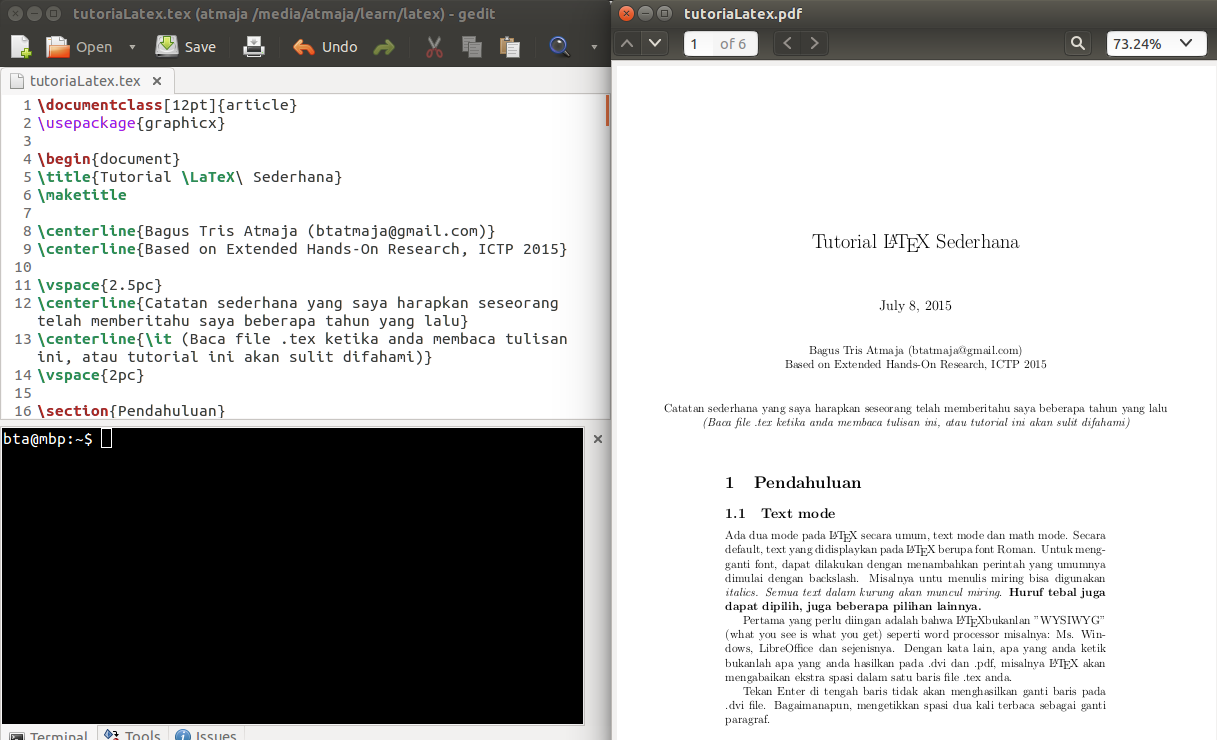
\includegraphics[width=4.2in]{pict/gedit-latex.png}
\end{center}
\caption{Tampilan Gedit dengan plugin Latex}
\end{figure}


\section{Pendahuluan}
\label{first}

\subsection{Text mode}


Ada dua mode pada \LaTeX\ secara umum, text mode dan math mode. Secara default, text yang didisplaykan pada \LaTeX\ berupa font Roman. Untuk mengganti font, dapat dilakukan dengan menambahkan perintah yang umumnya dimulai dengan backslash. Misalnya untu menulis miring bisa digunakan \textit{italics. Semua text dalam kurung akan muncul miring}. \textbf{Huruf tebal juga dapat dipilih, juga beberapa pilihan lainnya.}

Pertama yang perlu diingat adalah bahwa \LaTeX\ bukanlan "WYSIWYG" (what you see is what you get) seperti word processor misalnya: Ms. Windows, LibreOffice dan sejenisnya. Dengan kata lain, apa yang anda ketik bukanlah apa yang anda hasilkan pada .dvi dan .pdf, misalnya \LaTeX\ akan mengabaikan ekstra spasi dalam                   satu baris file .tex anda.

Tekan Enter
di
tengah
baris
tidak akan menghasilkan ganti baris pada .dvi file. Bagaimanapun, mengetikkan spasi dua kali terbaca sebagai ganti paragraf.

Misalnya seperti ini, double enter akan diabaikan, setelah double enter pertama. Dengan kata lain anda


tidak




dapat




menambahkan





spasi




antar 





baris, tidak peduli berapa kali anda menekan enter pada file .tex file.

Agar dapat menambahkan spasi vertikal anda perlu menambahkan perintah "vspace"; misalnya untuk menambahkan satu inchi spasi antar baris gunakan \verb|\vspace{1in}|, seperti ini:
\vspace{1in}

Untuk mendapatkan jarak antar baris 3 spasi gunakan,  \verb|\vspace{3pc}|
("pc" kependekan dari "pica", ), seperti berikut:
\vspace{3pc}

Perhatikan bahwa perintah \LaTeX\ selalu diawali dengan backslash. 
Beberapa perintah, seperti \verb|\vspace|, memerlukan argumen (disini, panjang) dalam kurung kurawal.

\subsection{Math mode}

Mode math adalah mode \LaTeX\ yang lain. Ini bisa dipilih dengan beberapa cara. Contohnya, text diantara tanda dolar diintepretasikan sebagai mode math, $g=4$. Formula matematika tersebut dapat ditambahkan didalam text. Pasangan tanda dolar ganda akan menghasilkan formulasi matematika dalam baris selanjutnya, $$g=4$$ Beberapa simbol dapat diakses seperti $\alpha$. Persamaan standar dapat dibentuk dengan, misalnya $\phi=x+2$.

Mode matematika adalah kekuatan \LaTeX\ yang sesungguhnya, yang membedakannya dengan word processor. Dengan \LaTeX\ kita bisa menulis persamaan matematika dengan sangat cantik yakni dengan menggunakan tanda \verb|$|.
Contoh lain misalnya, $2x^3 - 1 = 5$ ditulis dengan \verb|$2x^3 - 1 = 5$|. 

Contoh yang lebih menarik adalah menuliskan limit. Misalnya dengan menampilkan persamaan baru ditengah sebagai berikut,

$$\lim_{N \to \infty} \sum_{k=1}^N f(t_k) \Delta t.$$

Jika anda tidak ingin persamaan tersebut berada di tengah, namun anda ingin menampilkan dengan baik semuanya, gunakan  \verb|\displaystyle| dan untuk menampilkan dalam baris gunakan  $\displaystyle \lim_{N \to \infty} \sum_{k=1}^N f(t_k) \Delta t.$  Tentu saja ini akan menambah jarak spasi pada baris tersebut beberapa cm/inch. Untuk menambahkan nomor persamaan, anda dapat menggunakan \verb|\begin{equation}| seperti berikut,

\begin{equation}
    e=mc^2
\label{einstein1} 
\end{equation}

Untuk menyitasi/merefer persamaan \ref{einstein1} anda bisa menggunakan \verb|\label{}| dan memanggilnya dengan \verb|\ref{}| seperti pada persamaan \ref{einstein1} diatas. Penulisan persamaan \ref{einstein1} diatas menggunakan environenment yang akan dibahas pada \ref{enviro}.


Selain text dan persamaan matematika, ada banyak yang bisa kita lakukan dengan \LaTeX\, misalnya untuk membuat tabel, diagram, gambar persamaan bernomor, label, matriks, dll. Anda dapat mengatur batas kanan-kiri, atas-bawah, spasi, alignment,  {\it et cetera} dengan tingkat akurasi yang tinggi dibanding dengan penglihatan manusia. Dengan word processor, anda akan menghabiskan banyak waktu, tapi tidak bila anda menguasai \LaTeX.

Cara belajar \LaTeX\ adalah dengan mencoba berbagai contoh. Carilah beberapa contoh file .tex files, lihat bagiamana output pdf yang dihasilkan, bagaimana menghandle gambar dan memodifikasi apa yang anda inginkan. Ada banyak template \LaTeX\ yang bisa dicoba, dan biasanya jurnal dan conference menyediakan template untuk kegiatan mereka.


\subsection{Cross-Referencing}
\label{subref}

Latex dapat menghandle cross-reference section dan subsection. Misalnya, pada section pertama direfensikan sebagai section \ref{first} dan subsection ini akan direferensikan dengan \ref{subref}.


\subsection{Environments}
\label{enviro}
Hal kedua terpenting dalam \LaTeX\ adalah bahwa anda mengetikkan dalam suatu "environments" yang mirip dengan pemrograman. 
Sampai saat ini kita menggunakan text reguler (kecuali sudah kita perkaya dengan  \verb|\verb| huruf miring, tebal dll).  Ada dua cara untuk masuk dan keluar dari "environment", yakni secara langsung dengan kurung kurawal atau dengan "begin" dan "end".
\vspace{1pc}

\centerline{Ini adalah cara pertama...}

\begin{center}
Ini adalah cara kedua.
\end{center}

\noindent Sebenarnya ada cara lain yang digunakan sebagaimana contoh di atas. Misalnya,
{\sc seperti ini}. Cara anda masuk dan keluar bergantung pada jenis "environment" yang anda gunakan; misalnya anda menggunakan\verb|\underline| "diluar" dan \verb|\it| "didalam"; 
perhatikan \underline{ini} versus {\it ini}.



Perhatikan pada cara kedua, environment dibuka dengan \texttt{begin} dan diakhiri dengan pernyataan \texttt{end}.

Contoh untuk persamaan matematika,
\begin{equation}
\phi=2+x
\end{equation}
Contoh di atas tidak menggunakan dolar ataupun dolar ganda karena menggunakan environment \texttt{equation}.

Contoh lain,
\begin{center}
text akan diletakkan di tengah.
\end{center}



Gambar juga dapat dimasukkan dalam environment, yakni dengan \texttt{figure}.
\begin{figure}
\begin{center}
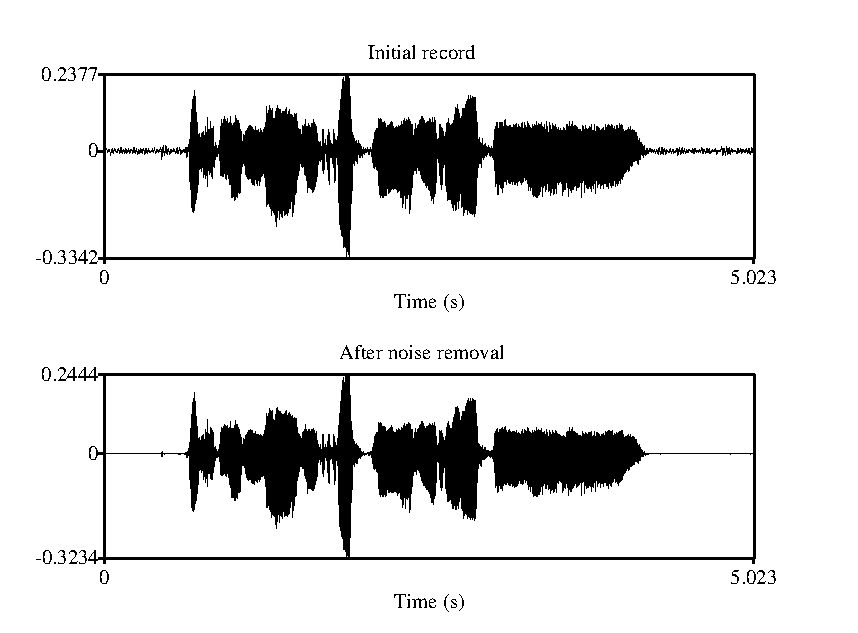
\includegraphics[width=3.2in]{pict/praat.eps}
\end{center}
\caption{detail caption gambar}
\end{figure}

Misalnya anda dapat menggunakan sembarang gambar untuk dimasukkan pada latex. Format gambar yang dapat disertakan dalam \LaTeX\ paling baik adalah dalam format \texttt{.eps}. Format lain bisa disertakan, namun akan lebih \textit{tricky}. Untuk bisa menyertakan gambar, anda harus menambahkan packages graphicx (baris 2 .tex).


Setiap environment bisa diberi label untuk memudahkan cross-reference,
\begin{equation}
\label{simple}
2x=4
\end{equation}
Persamaan \ref{simple} hasilnya adalah $x=2$.


\subsection{Sub dan superscripts}
Untuk menampilkan subscript dan superscript kita bisa menggunakan tanda underscore dan eksponen. Contohnya luas dari lingkaran adalah $\pi r^2$.  Jika anda menuliskan $\pi ^{r2}$, maka akan terjadi error. Begitu juga dengan subscripts, dapat ditulis dengan $\phi_{bgd}$. 

\section{Classes dan packages}
Ada file opsional yang dapat di-load dalam dokumen. Sebuah file \texttt{*.cls} atau class file pada baris pertama dan mengotrol bentuk file, mirip dengan css pada HTML (banyak kemiripan antara HTML dan TEX). Sebuah file  \texttt{*.sty} atau file style, biasanya diload pada \LaTeX\ seperti berikut,
\begin{verbatim}
\documentclass[twocolumn,amsmath,amssymb,floatfix]{ revtex4}
\usepackage{amssymb}
\usepackage{amsmath}
\usepackage[dvips]{graphicx}
\end{verbatim}

Baris pertama meload class \textit{revtex}. Ini biasanya digunakan untuk persiapan jurnal, dan setiap jurnal biasanya menyediakan file .sty nya. File \texttt{sty} diasosiasikan dengan beberapa simbol matematika dan untuk menghandle gambar. Jika anda mengubah baris pertama dengan perintah lain, maka keseluruhan format dokumen akan berubah secara total, misalnya dari satu kolom menjadi dua kolom.

\section{Membuat List}
Salah satu teknik penting dalam penulisan adalah dengan memaparkan poin per poin atau yang dikenal dengan list, baik bullet maupun numbering.

Unordered list, Contoh:
\begin{itemize}
\item Ini adalah unordered list pertama
\item Ini adalah unordered list kedua
    \begin{itemize}
    \item Ini adalab sub-list pertama
    \item ini adalah sub-list kedua
    \end{itemize}
\end{itemize}

Ordered list, Contoh:
\begin{enumerate}
\item Ini adalah ordered list pertama
\item Ini adalah ordered list kedua
    \begin{enumerate}
    \item Ini adalab sub-list pertama
    \item ini adalah sub-list kedua
    \end{enumerate}
\item Ini adalah ordered list ketiga \ldots
\end{enumerate}

\section{Membuat Tabel}
Contoh tabel sederhana dapat dibuat dengan perintah berikut,
\begin{verbatim}
\begin{tabular}{ l c r }
  1 & 2 & 3 \\
  4 & 5 & 6 \\
  7 & 8 & 9 \\
\end{tabular}
\end{verbatim}
Hasilnya adalah sebagai berikut,\\
\begin{tabular}{ l c r }
  1 & 2 & 3 \\
  4 & 5 & 6 \\
  7 & 8 & 9 \\
\end{tabular}
\\
\\
By default, tabel pada latex akan menempatkan teks anda di tengah, jika yang anda masukkan berupa gambar, maka gunakan perintah berikut agar vertically centered.
\begin{verbatim}
\raisebox{-.5\height}{\includegraphics[width=2in]{pict/m1}}
\end{verbatim}

\section{Menulis Limit dan Integral}
Untuk menuliskan limit, gunakan kode berikut,
\begin{verbatim}
$$\lim_{x\to a} f(x) = L$$ 
\end{verbatim}
Hasilnya adalah sebagai berikut, \\
$$\lim_{x\to a} f(x) = L $$
Jika kita menulisnya \emph{inline} dengan single \$ maka hasilnya adalah seperti ini:
$\lim_{x\to a} f(x) = L$
Untuk integral,


\section{Berbagai tanda kurung dan ukurannya}
By default, kita sering menggunakan tanda kurung "(...)" pada ukuran normal, namun untuk persamaan berupa fraksi atau pembagian, kita membutuhkan tanda kurung dengan ukuran yang lebib besar, caranya adalah sbb,
\begin{verbatim}
$\bigl( xxx \bigr)$
$\Bigl[ xxx \Bigr]$
$\biggl\{ xxx \biggr\}$
$\Biggl| xxx \Biggr|$
\end{verbatim}
Hasilnya adalah sbb:\\
$\bigl( xxx \bigr)$ \\
$\Bigl[ xxx \Bigr]$  \\
$\biggl\{ xxx \biggr\}$ \\
$\Biggl| xxx \Biggr|$ 

\section{Bibliography}
Ada banyak cara untuk memasukkan bibliography atau referensi. Cara yang paling sederhana adalah dengan menggunakan environment yang disebut \texttt{thebibliography}.  Namun, untuk memudahkan manajemen referensi (untuk banyak referensi) biasanya orang menggunkankan BibTeX, yang mengatur sitasi sendiri secara terpisah dalam format file \texttt{*.bib}.  Sitasi dapat ditambahkan dengan: \cite{langer1989}.

\begin{thebibliography}{9}

\bibitem{langer1989} Ernest Langer, \textit{The importance of being earnest}, J.\ Irrepr.\ Results \textbf{17} (1989), 101--102.

\end{thebibliography}


\end{document}
